\documentclass{IEEEcsmag}

\usepackage[colorlinks,urlcolor=blue,linkcolor=blue,citecolor=blue]{hyperref}
\expandafter\def\expandafter\UrlBreaks\expandafter{\UrlBreaks\do\/\do\*\do\-\do\~\do\'\do\"\do\-}
\usepackage{upmath,color}
\usepackage{graphicx}
\usepackage{amsmath,amssymb}
\usepackage{seqsplit}
\usepackage{tikz}
\usepackage{lettrine}
\usetikzlibrary{positioning,arrows.meta,calc}

% --- Fallbacks for macros some IEEEcsmag forks omit (DanySK template) ---
\providecommand{\jtitle}[1]{}
\providecommand{\chapteri}[1]{\lettrine[lines=2,findent=2pt,nindent=0pt]{#1}{}}

% --- Math shortcuts ---
\newcommand{\Fr}{\mathbb{F}_r}
\newcommand{\Gone}{\mathbb{G}_1}
\newcommand{\Cold}{C_{\mathsf{old}}}
\newcommand{\Cnew}{C_{\mathsf{new}}}
\newcommand{\eold}{\epsilon_{\mathsf{old}}}
\newcommand{\snew}{s_{\mathsf{new}}}
\newcommand{\Rmem}{R_{\mathsf{Mem}}}
\newcommand{\Rupd}{R_{\mathsf{Upd}}}

% --- Magazine metadata (placeholders for editor to fill in) ---
\jvol{XX}
\jnum{XX}
\paper{1}
\jmonth{April}
\jname{IEEE Security \& Privacy}
\jtitle{IEEE Security \& Privacy}
\pubyear{2026}

\setcounter{secnumdepth}{0}

\begin{document}

\sptitle{Feature Article: Privacy and Cryptography}

\title{Postmortems from a SNARK-Gated Group Registry on Stellar}

\author{Rinat Enikeev}
\affil{Independent researcher, Tallinn, Estonia}

\markboth{FEATURE ARTICLE}{FEATURE ARTICLE}

\begin{abstract}Pushing group-membership metadata onto a public ledger eliminates the trusted server but introduces new failure modes. This article reports two postmortems from a zero-knowledge-gated registry deployed on a public blockchain: a soundness theorem that bound the wrong predicate, and a privacy invariant that lived only in a Security Considerations bullet.

\vspace{4pt}\noindent\textbf{Index Terms}---Authentication, blockchains, cryptographic protocols, privacy, smart contracts, zero-knowledge proof.
\end{abstract}

\maketitle


\chapteri{M}essaging content is routinely end-to-end encrypted; membership metadata almost never is. Every mainstream architecture we know of has at least one application-layer operator---a server, a federated peer, a Delivery Service~\cite{rfc9420}---positioned to observe who is in which group. Signal's Private Group System~\cite{chase2020} shows this can be closed to an honest-but-curious operator using anonymous credentials.

Onym asks a narrower question: can the \emph{registry} that records a group's current membership state be pushed onto a public ledger with a SNARK-gated authorization rule, so that no application-layer operator sits in the metadata path at all? The answer we report on is ``yes, with substantial caveats''---and the caveats are the most useful part of what follows.

We want to set reviewer expectations directly. This is a registry-primitive experience report, not:
\begin{itemize}
\item \emph{a messaging substrate paper}---the MLS-side integration is future work and we do not claim to have built it.
\item \emph{a cryptographic-proofs contribution}---the Construction section states what the SNARK binds in the minimum formality the postmortems need; readers who want full simulation-extractability definitions should consult~\cite{baghery2021,lipmaa2019,fuchsbauer2018agm}.
\item \emph{a production-readiness claim}---the deployment is alpha on testnet, and the Limitations section says so plainly.
\item \emph{a general-policy paper}---only the unanimous-member mode is analyzed; other policies shipped in v1.7.0 on 2026-04-19 and are not reviewed here.
\end{itemize}

The contribution is the engineering postmortems and the design-review template that fell out of them.

\section{CONSTRUCTION}

Let $\Fr$ be the BLS12-381 scalar field and $G_1 \in \Gone$ a generator. Let $H$ denote Poseidon~\cite{grassi2021} at the standard BLS12-381 parameter set. For a member set $S = \{\mathsf{pk}_1, \ldots, \mathsf{pk}_n\}$ canonicalized under compressed-G1 serialization, let $\mathsf{root}(S)$ be the Poseidon Merkle root with leaves $H(\mathsf{pk})$. The group commitment is
\begin{equation}
C = H\!\bigl(H(\mathsf{root}(S), \epsilon),\, s\bigr) \in \Fr,
\end{equation}
where $\epsilon$ is the epoch counter and $s$ is a per-epoch salt uniform in $\Fr$. The nested structure is not cosmetic: the inner digest $H(\mathsf{root}, \epsilon)$ is what sub-circuits bind to when they need to reference ``this group at this epoch'' without disclosing $s$, and keeps the salt-disclosure story orthogonal to root-or-epoch disclosure across related proofs.

Two Groth16 relations~\cite{groth2016}, both proved on BLS12-381:
\begin{itemize}
\item $\Rmem(C, \epsilon)$: prover knows a secret key $sk$, a Merkle path, and the salt $s$ opening $C$ to a tree containing $H(sk \cdot G_1)$.
\item $\Rupd(\Cold, \eold, \Cnew)$: $\Rmem$ holds at $(\Cold, \eold)$, and $\Cnew$ is an opening-commitment under epoch $\eold + 1$ with a fresh salt $\snew$.
\end{itemize}

Crucially, $\Cnew$ is a public input to $\Rupd$---part of what the proof binds, not a contract-controlled parameter. Getting this wrong was P1.

\subsection{What the SNARK Binds, Informally}

Simulation-extractability (SE)---not plain knowledge-soundness---is the right property here, because Groth16 is malleable~\cite{grothmaller2017}: an adversary can reshape an honest proof into a different accepting proof without a witness. Under SE (in the algebraic group model plus random-oracle heuristic for out-of-circuit Poseidon), any accepting $\Rupd$ proof implies the submitter knows a witness linking the old commitment to the new one via a current member's key, even if the submitter has previously observed simulated proofs. The public-input-hashing modification~\cite{baghery2021} (building on prior work~\cite{lipmaa2019}) is what makes SE available for Groth16; the deployed contract uses it.

We do not write the formal games here. The genre of this paper does not require them, the minimal content needed for the postmortems is the paragraph above, and the reader who wants the proofs should go to the cited work~\cite{baghery2021,lipmaa2019,fuchsbauer2018agm} where they are already written.

\subsection{Replay}

The contract entry point checks that the submitted $(\Cold, \eold)$ match stored state before writing $\Cnew$ and incrementing the epoch. This is a contract-level invariant enforced by our entry-point code, not a cryptographic property. A proof captured off-wire has authorization power at most until the next legitimate update wins the first-write race.

\subsection{Fee-Payer Unlinkability, Stated Cleanly}

Onym's on-chain footprint is information-theoretically independent of which group member authored the update; all unlinkability loss is attributable to side channels outside the ledger. We claim no more than that, and we claim no less. For $n \geq 3$ this is a useful guarantee under reasonable operational assumptions about the relayer; for $n = 2$ it is trivially defeated by realistic auxiliary observations, which is why Onym is a group substrate and not a 1:1 substrate.

\subsection{Deployment Honesty}

The deployed verification keys are the output of a single-contributor Phase-2 setup. Against the setup operator---the party holding the aggregate simulation trapdoor---the authorization property is vacuous, because that party can forge an accepting proof for any public input including hostile state rewrites. A multi-contributor Phase-2 MPC is the first production-readiness item. We publish these postmortems before that ceremony has been re-run because the lessons are about the engineering missteps that preceded it, not claims about the current deployment's guarantees.


\section{IN PLAIN LANGUAGE}

Picture a town hall keeping one sealed envelope per club. The envelope reveals nothing about members. When a member wants to act on the club's behalf, they hand over a slip proving they belong inside the envelope without anyone opening it. When the club changes, one member writes what the next envelope should say, proves ``I belong inside yesterday's envelope and today's envelope is the correct next version of it,'' and the hall swaps envelopes. Nothing on the hall's wall ever names a member.

The hall is the Stellar blockchain. The envelope is a 32-byte Poseidon commitment. The slip is a 192-byte Groth16 proof. The arithmetic check is three BLS12-381 pairings run by a Soroban smart contract. The member's secret is a BLS12-381 private key on their device. Figure~\ref{fig:arch} shows the full path.

Three things leak despite the envelope. (i) Someone pays the transaction fee; if members paid their own, their Stellar accounts would be linked to group activity, so Onym submits through a public relayer that pays from its own account. The relayer knows which group, when, and who asked---a metadata observation point we do not close. (ii) Each group is created inside a size tier ($\leq$ 32, $\leq$ 256, or $\leq$ 2048 members) which is public; crossing a tier is a monotonic public disclosure. (iii) Stellar validators see the relayer's submission before the network does, on a seconds-scale window around block close.

\begin{figure*}[t]
\centering
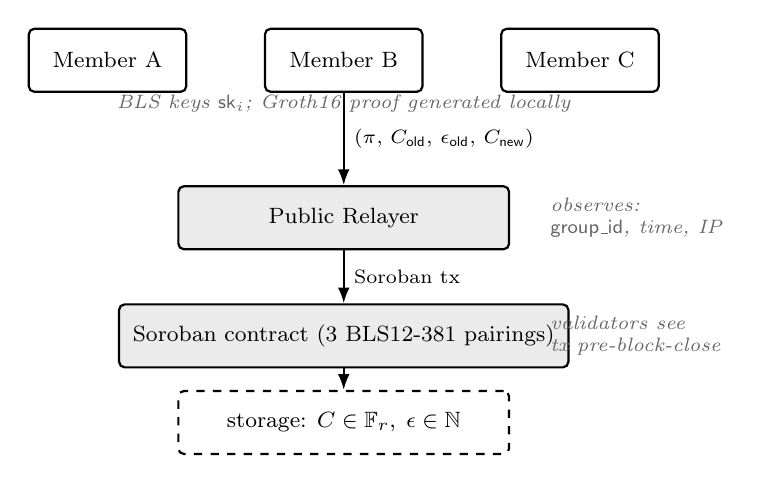
\begin{tikzpicture}[
    font=\footnotesize,
    box/.style={draw, thick, rounded corners=2pt, inner sep=5pt, align=center, minimum height=8mm},
    arr/.style={-{Latex[length=2mm]}, thick},
    leak/.style={font=\scriptsize\itshape, color=black!60, align=left}
]

% Members
\node[box, minimum width=20mm] (mA) at (-3,0) {Member A};
\node[box, minimum width=20mm] (mB) at (0,0) {Member B};
\node[box, minimum width=20mm] (mC) at (3,0) {Member C};
\node[font=\scriptsize\itshape, color=black!60] at (0,-0.55) {BLS keys $\mathsf{sk}_i$; Groth16 proof generated locally};

% Relayer
\node[box, fill=black!8, minimum width=42mm] (relay) at (0,-2.0) {Public Relayer};
\node[leak, anchor=west] at (2.5,-2.0) {observes:\\$\mathsf{group\_id}$, time, IP};

% Contract
\node[box, fill=black!8, minimum width=42mm] (chain) at (0,-3.5) {Soroban contract (3 BLS12-381 pairings)};
\node[leak, anchor=west] at (2.5,-3.5) {validators see\\tx pre-block-close};

% Storage
\node[box, dashed, minimum width=42mm] (store) at (0,-4.6) {storage: $C \in \mathbb{F}_r,\; \epsilon \in \mathbb{N}$};

% Arrows
\draw[arr] (mB.south) -- node[right, font=\scriptsize] {$(\pi,\, \Cold,\, \eold,\, \Cnew)$} (relay.north);
\draw[arr] (relay.south) -- node[right, font=\scriptsize] {Soroban tx} (chain.north);
\draw[arr] (chain.south) -- (store.north);

\end{tikzpicture}
\caption{Onym data and metadata flow. Each member holds a BLS12-381 secret key and produces a 192-byte Groth16 proof $\pi$ locally; one member submits the update tuple via a public relayer that pays the transaction fee. The Soroban contract verifies the proof using three BLS12-381 pairings and writes the new 32-byte commitment $\Cnew$ and incremented epoch to storage. Italicized callouts mark the metadata each non-member party in the path observes.}
\label{fig:arch}
\end{figure*}


\section{POSTMORTEMS}

\subsection{P1---The Theorem That Proved the Wrong Thing}

\textbf{Severity.} Critical authorization vulnerability: any party in the network path between a prover and the contract could substitute the new commitment written to storage while retaining the prover's still-valid proof. Every privacy and authorization guarantee was void for the operation that changes group state.

\textbf{What went wrong.} Through v1.2.9 every state-changing operation shared one circuit with relation $\Rmem$ and public inputs $(C, \epsilon)$. The \texttt{update\_commitment} entry point accepted a separate \texttt{new\_commitment: BytesN<32>} parameter that the contract wrote to storage. The proof authorized knowledge of a member in the \emph{current} state; it said nothing about which next state was being authorized. \texttt{new\_commitment} was a contract-controlled free parameter.

\begin{figure*}[t]
\centering
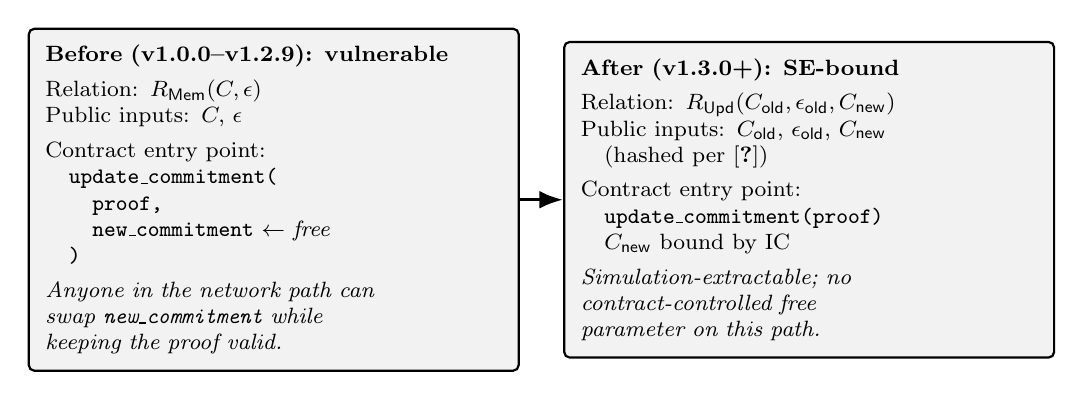
\begin{tikzpicture}[
    font=\footnotesize,
    panel/.style={draw, thick, rounded corners=2pt, inner sep=6pt, text width=58mm, align=left, fill=black!5},
    arr/.style={-{Latex[length=3mm]}, very thick}
]

\node[panel] (before) at (-3.4,0) {%
    \textbf{Before (v1.0.0--v1.2.9): vulnerable}\\[3pt]
    Relation: $\Rmem(C, \epsilon)$\\
    Public inputs: $C,\, \epsilon$\\[3pt]
    Contract entry point:\\
    \quad\texttt{update\_commitment(}\\
    \quad\quad\texttt{proof,}\\
    \quad\quad\texttt{new\_commitment} $\leftarrow$ \emph{free}\\
    \quad\texttt{)}\\[3pt]
    \emph{Anyone in the network path can\\swap \texttt{new\_commitment} while\\keeping the proof valid.}
};

\node[panel] (after) at (3.4,0) {%
    \textbf{After (v1.3.0+): SE-bound}\\[3pt]
    Relation: $\Rupd(\Cold, \eold, \Cnew)$\\
    Public inputs: $\Cold,\, \eold,\, \Cnew$\\
    \quad(hashed per~\cite{baghery2021})\\[3pt]
    Contract entry point:\\
    \quad\texttt{update\_commitment(proof)}\\
    \quad$\Cnew$ bound by IC\\[3pt]
    \emph{Simulation-extractable; no\\contract-controlled free\\parameter on this path.}
};

\draw[arr] (before) -- (after);

\end{tikzpicture}
\caption{P1: the bug and its fix. The original relation $\Rmem$ bound only the current state $(C, \epsilon)$; the contract wrote whatever \texttt{new\_commitment} appeared in the call, leaving it controllable by anyone in the network path. The fix promotes $\Cnew$ to a public input of a new relation $\Rupd$, and the public-input-hashing modification of~\cite{baghery2021} adds simulation-extractability so the proof cannot be re-randomized into a different accepting proof.}
\label{fig:p1}
\end{figure*}

\textbf{Who caught it.} An external reviewer, contracted for a Groth16-circuit-to-contract-ABI seam pass, asked: \emph{``Where in the math is the argument that this proof is non-transferable to a different \texttt{new\_commitment}?''} The answer was: nowhere. A proof binds to its public inputs and nothing else~\cite{groth2016,lipmaa2019}. A second subtlety surfaced during the fix: even once $\Cnew$ is a public input, plain Groth16 is malleable~\cite{grothmaller2017}, so what is needed is simulation-extractability, not plain knowledge-soundness. Making $\Cnew$ an IC input was necessary but not sufficient until the public-input-hashing modification~\cite{baghery2021} was added.

\textbf{Why four preceding reviews did not catch it.} The system had passed four structured reviews---circuit soundness, contract ABI, primitive choice, wire-format correctness---each well-scoped within itself. The seam that failed was \emph{between} scopes: no pass owned the question of whether the operation's security predicate was expressible in terms of the statement the proof actually bound. The lesson is about review topology, not individual reviewers.

\textbf{Fix and lesson.} Split the relation---$\Rmem$ unchanged, $\Rupd$ new with $(\Cold, \eold, \Cnew)$ public, public inputs hashed per the modification of~\cite{baghery2021} to obtain SE (Figure~\ref{fig:p1}). The deployed contract was re-read by the same external reviewer after the fix. Formal soundness of a relation says nothing about the security of an operation whose security predicate is over variables the relation does not mention. Our design-review template now requires, per authorized operation: (1) a one-sentence predicate stating what the proof binds; (2) an enumeration of every value the contract reads on that path, labeled \emph{in IC} or \emph{contract-controlled}; (3) a side-by-side read of the relation file and the contract entry-point; (4) an explicit statement of whether knowledge-soundness or simulation-extractability is the intended level.

\subsection{P2---Transport-Layer Co-Membership Leakage}

Onym's clients exchange invitations and ciphertext over Nostr relays. Each Nostr event is signed by a secp256k1 key. Through v1.2.7 each client signed every event with its \emph{long-lived} identity key. A companion transport spec mentioned the implication in one bullet of its Security Considerations:

\begin{quote}
\emph{``Stable Nostr device keys improve usability but increase sender linkability.''}
\end{quote}

Technically true, strategically misleading: the actual consequence was \emph{group linkability}---any relay could cluster the user base by co-membership from public relay data, ``these $N$ keys all published to hidden-topic $T \to$ these $N$ devices are in the same group.''

\textbf{Fix.} Ephemeral per-event secp256k1 keys; topic tags now derived per-epoch as $H(\mathsf{group\_id} \mathbin\| \epsilon)$ and rotated on every state change; a receive-side audit moved four code paths from \texttt{event.pubkey} to the inner BLS public key. We do not claim that no traffic-analysis-based co-membership inference remains---relay-level timing correlation is an open residual channel and also feeds the fee-payer side-channel story discussed earlier.

\textbf{Lesson.} A privacy invariant that lives in a \emph{Security Considerations} bullet of a different document is fiction. Identity coupling---one key serving as both signing key and sender identity---is a recurring antipattern; decoupling is almost free on day one and a postmortem otherwise.

\subsection{A Demoted Lesson: Host-Function Hashes as a Constraint-Budget Landmine}

An earlier version of Onym composed Poseidon inside the circuit with SHA-256 outside, chosen because Soroban exposes SHA-256 as a native host function. Because the circuit must reproduce the outer hash to bind its inner Poseidon output to the commitment the contract observes, the outer primitive's R1CS cost is paid in full at proving time: one SHA-256 compression requires approximately 25{,}000 R1CS constraints in the standard arkworks gadget, which dominated the small-tier circuit by an order of magnitude. Replacing the outer SHA-256 with two Poseidon calls (approximately 600 constraints in total) reduced R1CS cost by 8--14$\times$ across tiers.

The durable takeaway---\emph{R1CS cost dominates host-function cost for any primitive that straddles the circuit boundary}---is what the design-review template retains. The specific SHA-256-versus-Poseidon trade-off that produced the mistake is now moot on Stellar: Protocol 25's CAP-0075 (January 2026) adds native Poseidon and Poseidon2 host functions, collapsing the host-side asymmetry that made SHA-256 the attractive default.


\section{EVALUATION}

Testnet deployment in alpha phase. Contract: \texttt{\seqsplit{CC6NUUKG25RSFI6D57HISDQ4HRBLXFAUC3GFVZIACHQX3NLRPYTRWWKE}} on Stellar testnet. Source: \url{https://github.com/rinat-enikeev/stellar-mls}. Postmortem tag ranges: P1 pre-fix at tags \texttt{v1.0.0}--\texttt{v1.2.9}; P2 pre-fix at tag \texttt{v1.2.7}; multi-policy landing at tag \texttt{v1.7.0} (2026-04-19). Groth16 proofs are 192 bytes; public inputs add 32 bytes for $\Rmem$ and 96 bytes for $\Rupd$. On-chain verification invokes three BLS12-381 pairings plus a small multi-scalar multiplication; Soroban instruction count is 6--10M per update, inside testnet fee budgets. We do not report production group counts or update volumes; the system is not in production.

What an observer learns, once an honest multi-contributor Phase-2 MPC has been run (a deployment prerequisite, currently unmet): that a group exists, how many state changes have occurred and when, its current size tier and any prior tier it graduated out of, and the relayer's identity. Not learned: the member set, the updater's identity, the exact count within tier, or whether the group shrank or rotated within tier. We have not performed a formal differential-privacy analysis of the timing channel nor quantified tier-transition information leakage; methodology and measurements are future work.


\section{LIMITATIONS}

\begin{itemize}
\item \textbf{Single-contributor Phase-2 setup.} Restated here because it is the gating limitation for every authorization claim. Until this is redone as a multi-contributor MPC, the deployment's guarantees are vacuous against the setup operator.
\item \textbf{Unanimous-member mode only.} A single current member can replace the entire set. That is the defining property of the mode; applications that cannot tolerate it need a different policy.
\item \textbf{Validator-set timing channel.} Seconds-scale observation window around block close; qualitatively weaker than an application server (no ability to decide which transactions exist, bounded retention), but not cryptographically absent.
\item \textbf{Fee-payer correlation via the relayer.} The relayer's account is a metadata observation point; a single relayer is better than each member being their own fee payer but worse than a decentralized pool. The relayer also learns submission timing and originating IP unless the member submits over a mixnet, neither of which Onym closes.
\item \textbf{All members must be online provers.} Delegating Groth16 proving to a server would reintroduce operator trust.
\item \textbf{Key compromise in unanimous mode.} A stolen member key authorizes arbitrary state transitions including expelling all other members. Recovery is a policy-layer question and is not solved here.
\item \textbf{MLS integration is a sketch, not a demonstration.} We do not claim to have integrated with a conforming MLS Delivery Service; Mafia~\cite{mafia2025} is the directly relevant prior work on the DS-metadata side of the problem and the plausible composition partner.
\item \textbf{Pair chats.} Not a supported use case, per the clean statement in the Construction section.
\item \textbf{Post-quantum.} BLS12-381 + Groth16 is not PQ-secure. Migration to a PQ-curve or transparent-setup system (e.g., PLONK/FRI-based) is a deferred design question.
\end{itemize}


\section{RELATED WORK}

Closest in construction is Semaphore~\cite{semaphore}: both anchor a commitment tree on a public ledger and verify membership with a Groth16 SNARK. Onym differs in that the tree commits to an \emph{evolving group-membership set} rather than a fixed anonymity set, and the authorization predicate is over state \emph{transitions} rather than single-statement membership. Signal PGS~\cite{chase2020} is the gold standard for metadata-private group membership under a trust-the-operator assumption; Onym occupies an adjacent design point (no application-layer operator, public-chain validator set as residual trust). Mafia~\cite{mafia2025} addresses the MLS-DS half of the metadata problem and would plausibly compose with Onym in a production stack.

We do not include a broader ZK-pool lineage table (Railgun, AZTEC, Nocturne, Azeroth, etc.) because none of those systems is a close comparable for a group-membership registry with transition authorization, and gesturing at them at the genre level does not help a reader who already knows the space.


\section{CONCLUSION}

The contribution is two postmortems and a design-review template, not a production system or a cryptographic proofs contribution. The engineering takeaways generalize: a relation's soundness theorem says nothing about operations whose security predicate is over variables the relation does not mention, and operation-binding over Groth16 needs simulation-extractability rather than plain knowledge-soundness; privacy invariants that live in \emph{Security Considerations} bullets of other documents are fiction; R1CS cost dominates host-function cost for primitives that straddle the circuit boundary. Readers should take the postmortems more seriously than the system.\vspace*{-8pt}


\section{ACKNOWLEDGMENTS}

We thank the Stellar Development Foundation for the ZK primitives landed in the chain core: CAP-0059~\cite{cap0059} (BLS12-381 host functions, Protocol 22, December 2024) made on-chain Groth16 verification feasible at this gas level and is what enabled this work, and the Protocol 25 \emph{X-Ray} track (mainnet activation January 22, 2026) added CAP-0074 (BN254) and CAP-0075 (Poseidon/Poseidon2), which together collapse the host-vs-circuit hash trade-off behind the demoted lesson and widen the curve and primitive design space for successors. We thank the arkworks contributors for the Rust Groth16 and Poseidon gadgets; and the external code reviewer whose P1-catching question is the reason P1 is a postmortem rather than a zero-day. The author's other significant interlocutor was Claude (Anthropic, 2026), whose role is described in the \emph{Use of Generative AI} note below rather than folded into the human-contributor list.

\textbf{Use of generative AI.} The author is a builder, not a cryptographer. Onym was designed, implemented, and deployed before any of the Construction section's language existed on paper. Turning the working system into writing that a cryptographer would read as sound required consulting Claude extensively---both as a tutor on the literature (AGM, simulation-extractability, the public-input-hashing modification, Poseidon's ROM framing) and as a reader whose hard critiques of successive drafts shaped the paper's framing: retitling away from an over-claim, committing to the registry-primitive genre rather than oscillating into messaging-substrate territory, and moving the Phase-2 MPC disclosure out of a limitations subsection and into the abstract. For each such framing change the author read the sources Claude surfaced and adopted it only after the sources checked out. This article is a builder's postmortems and review lessons, not a protocol proposal; the postmortems are the author's work, the author is accountable for every technical statement and any remaining errors, and the formal scaffolding around the postmortems is in the paper at all because AI made it accessible to a builder.


\def\refname{REFERENCES}

\begin{thebibliography}{99}

\bibitem{rfc9420}
R. Barnes et al., ``The messaging layer security (MLS) protocol,'' IETF, RFC 9420, 2023.

\bibitem{groth2016}
J. Groth, ``On the size of pairing-based non-interactive arguments,'' in \emph{Proc. Annu. Int. Conf. Theory Appl. Cryptographic Techn. (EUROCRYPT)}, 2016, pp. 305--326.

% NOTE: zcash reference removed — was uncited in body. Restore if you want it as background citation in Construction.
% \bibitem{zcash}
% D. Hopwood et al., ``Zcash protocol specification,'' Electric Coin Company, Version 2024.5.0, 2024.

\bibitem{semaphore}
Privacy \& Scaling Explorations, ``Semaphore protocol specification v4,'' 2024. [Online]. Available: \url{https://docs.semaphore.pse.dev/}

\bibitem{grassi2021}
L. Grassi, D. Khovratovich, C. Rechberger, A. Roy, and M. Schofnegger, ``Poseidon: A new hash function for zero-knowledge proof systems,'' in \emph{Proc. 30th USENIX Secur. Symp.}, 2021, pp. 519--535.

\bibitem{grothmaller2017}
J. Groth and M. Maller, ``Snarky signatures: Minimal signatures of knowledge from simulation-extractable SNARKs,'' in \emph{Proc. Annu. Int. Cryptol. Conf. (CRYPTO)}, 2017, pp. 581--612.

\bibitem{chase2020}
M. Chase, T. Perrin, and G. Zaverucha, ``The signal private group system and anonymous credentials supporting efficient verifiable encryption,'' in \emph{Proc. ACM SIGSAC Conf. Comput. Commun. Secur. (CCS)}, 2020, pp. 1445--1459.

% NOTE: barbulescu2019 reference removed — was uncited in body. Restore if you want it as a key-size estimate cite for BLS12-381 discussion.
% \bibitem{barbulescu2019}
% R. Barbulescu and S. Duquesne, ``Updating key size estimations for pairings,'' \emph{J. Cryptol.}, vol. 32, no. 4, pp. 1298--1336, 2019.

\bibitem{baghery2021}
K. Baghery, M. Kohlweiss, J. Siim, and M. Volkhov, ``Another look at extraction and randomization of Groth's zk-SNARK,'' in \emph{Proc. Int. Conf. Financial Cryptogr. Data Secur.}, 2021, pp. 457--475.

\bibitem{cap0059}
Stellar Development Foundation, ``CAP-0059: Host functions for BLS12-381,'' 2024. [Online]. Available: \url{https://github.com/stellar/stellar-protocol/blob/master/core/cap-0059.md}

\bibitem{lipmaa2019}
H. Lipmaa, ``Simulation-extractable SNARKs revisited,'' Cryptology ePrint Archive, Paper 2019/612, 2019. [Online]. Available: \url{https://eprint.iacr.org/2019/612}

\bibitem{fuchsbauer2018agm}
G. Fuchsbauer, E. Kiltz, and J. Loss, ``The algebraic group model and its applications,'' in \emph{Proc. Annu. Int. Cryptol. Conf. (CRYPTO)}, 2018, pp. 33--62.

\bibitem{mafia2025}
T. Melissaris et al., ``Private delivery services for messaging layer security (Mafia),'' in \emph{Proc. Annu. Int. Conf. Theory Appl. Cryptographic Techn. (EUROCRYPT)}, 2025.

\end{thebibliography}\vspace*{-8pt}


% =============================================================
% AUTHOR BIOGRAPHY
%
% NOTE on photo: IEEE CS Magazine production will composite
% your color headshot from the separately-uploaded photo asset
% (headshot.jpg, also in this directory). The IEEEcsmag.cls
% biography environment has a known incompatibility with
% \includegraphics in its optional argument, so the
% manuscript-PDF biography is rendered photoless. This matches
% the rendering of the original CsMag_template.pdf and is the
% expected production workflow — you upload headshot.jpg as a
% supplementary file in the ScholarOne portal and production
% places it during typesetting.
% =============================================================
\begin{IEEEbiography}{Rinat Enikeev}{\,}is an independent researcher based in Tallinn, Estonia. His current research interests include applied zero-knowledge cryptography, metadata-private messaging, and smart-contract security review methodology. He has built and deployed Onym, a SNARK-gated group registry on Stellar Soroban (\url{https://github.com/rinat-enikeev/stellar-mls}). Contact him at rinat.enikeev@gmail.com.
\end{IEEEbiography}

\end{document}
